%!TEX  root = main.tex
\chapter{Ingénierie Dirigée par les Modèles}
\label{ch:IDM}
 
\PartialToc

Dans le chapitre précédent, nous avons vu que les modèles utilisés pour l'EA,
bien qu'offrant l'abstraction nécessaire pour adresser la complexité de l'entreprise, sont le
plus souvent purement contemplatifs et ne permettent pas de mener une analyses automatisée et pertinente 
de la structure et du comportement d'une architectures d'entreprise. L'IDM se fait fort de traiter la problématique
des modèles purement contemplatifs dans le contexte du génie logiciel. Dès lors, nous nous intéressons dans ce chapitre 
aux modèles, méthodes et techniques de l'IDM qui peuvent bénéficier à l'EA.


Ce chapitre présente ainsi la genèse et les objectifs de l'IDM dans la section~\ref{sec:genese_idm} avant 
d'en présenter les concepts fondamentaux que sont les modèles et les métamodèles
dans la section~\ref{sec:concepts_idm}. Dans une approche IDM, l'automatisation de la manipulation des modèles passe en premier
lieu par les techniques de transformation de modèle que nous introduisons dans la section~\ref{sec:transfo_idm}. Enfin, nous considérons
les approches d'EA existantes qui recourent à l'IDM et nous en dressons les contributions et les limites dans la section~\ref{sec:idm_for_ea}. 

\section{Genèse et objectifs}
\label{sec:genese_idm}

L'\gls{idm} est née du constat que le paradigme du «~tout est objet~», prôné dans les années 1980, a atteint ses limites avec ce début de siècle~\cite{greenfield2004software}. En effet, face à la croissance de la complexité des systèmes logiciels, au coût de la main d'œuvre et de la maintenance, une approche centrée sur le code, jugé alors seul représentant 
fiable du système, suscitait de moins en moins l'adhésion des industriels et du 
milieu académique. 

Partant de ce constat, l'\gls{omg} a proposé en novembre 
2000, l'approche \gls{mda} qui s'inscrit dans le cadre 
plus général de l'\gls{idm} et se réalise autour d'un certain nombre de standards tels 
qu'UML, \gls{mof}, XML, QVT, etc. Le monde de la recherche s'y est aussitôt intéressé 
pour dégager les principes fondamentaux de l'\gls{idm} 
\cite{bezivin2001towards, kent2002model, de2002using} et déjouer le 
piège des définitions parfois trop floues qui mènent à confondre les 
concepts du paradigme objet et ceux de l'\gls{idm}~\cite{bezivin2004search}. Par 
ailleurs, des industriels comme \gls{ibm}~\cite{booch2004mda} et Microsoft 
\cite{greenfield2004software} ont aussi rendu publique leur vision de l'\gls{idm}. 
Ainsi, l'\gls{idm} prend son origine dans la convergence de toutes ces visions et des 
avancées techniques de chacun.

L'originalité de l'\gls{idm} ne réside pas dans le recours systématique aux modèles 
pour le développement logiciel comme le laisserait entendre sa terminologie  
\cite{bezivin2004rapport}. Plusieurs méthodes de modélisation, telles que Merise 
ou SSADM, préconisent aussi l'utilisation de modèles mais dont le rôle s'achève aux 
phases amont du développement logiciel~: l'analyse et la conception. Les modèles 
servent alors à faciliter la communication et la compréhension entre les différents 
acteurs mais n'interviennent pas dans la phase de production, de maintien et 
d'évolution. Nous parlons dans ce cas de modèles «~contemplatifs~». 

L'\gls{idm} a pour objectif de rendre les modèles «~productifs~» sur tout le cycle de 
vie du système et à tous les niveaux d'abstraction. Pour y parvenir, les modèles 
doivent être décrits formellement afin d'être interprétés et exécutés par une 
machine. Dès lors, ces modèles permettent d'industrialiser la production 
logicielle, jusque-là centrée sur le code produit par l'informaticien 
\cite{bezivin2005unification}.



\section{Concepts fondamentaux}
\label{sec:concepts_idm}

En mettant à profit des disciplines telles que la modélisation par objets, 
l'ingénierie des langages, la compilation de langages, les méthodes formelles 
ou encore la programmation par composants, l'\gls{idm} offre un cadre intégrateur reposant 
sur quelques concepts fondamentaux : la notion de modèle et la relation 
\textit{Représente}, la notion de métamodèle et la relation 
\textit{ConformeÀ}.

\subsection{Modèle et Représentation}
La notion de modèle est centrale dans l'\gls{idm} car, comme nous venons de l'évoquer, 
l'enjeu de cette approche est de rendre les modèles productifs sur tout le cycle 
de vie du système. Il n'existe pas de définition universelle de la notion de 
modèle. En nous appuyant sur les définitions données dans les travaux 
\cite{minsky1967computation} \cite{bezivin2001towards} et 
\cite{seidewitz2003models}, nous adoptons la définition suivante du terme modèle~:
\\\

\begin{definition}
Un modèle est une abstraction d'un système, selon le bon point de vue, qui 
permet de répondre à des questions prédéfinies sur ce système en lieu et place 
de celui-ci.
\end{definition}

De cette définition découle la première relation fondamentale de l'\gls{idm} qui lie 
le modèle et le système qu'il représente. Celle-ci est nommée 
\textit{Représente} et notée $\mu$. Bien que la relation 
\textit{Représente} ne soit pas nouvelle dans l'ingénierie logicielle 
(Merise, UML), l'\gls{idm} a permis d'en définir les contours \cite{atkinson2003model} 
\cite{seidewitz2003models} \cite{bezivin2004search}.

\begin{figure}[!ht]
    %_BUILD_FULL \begin{center}\begin{tikzpicture}
    \node[inner sep=4pt] (photo) at (5,-1.86) {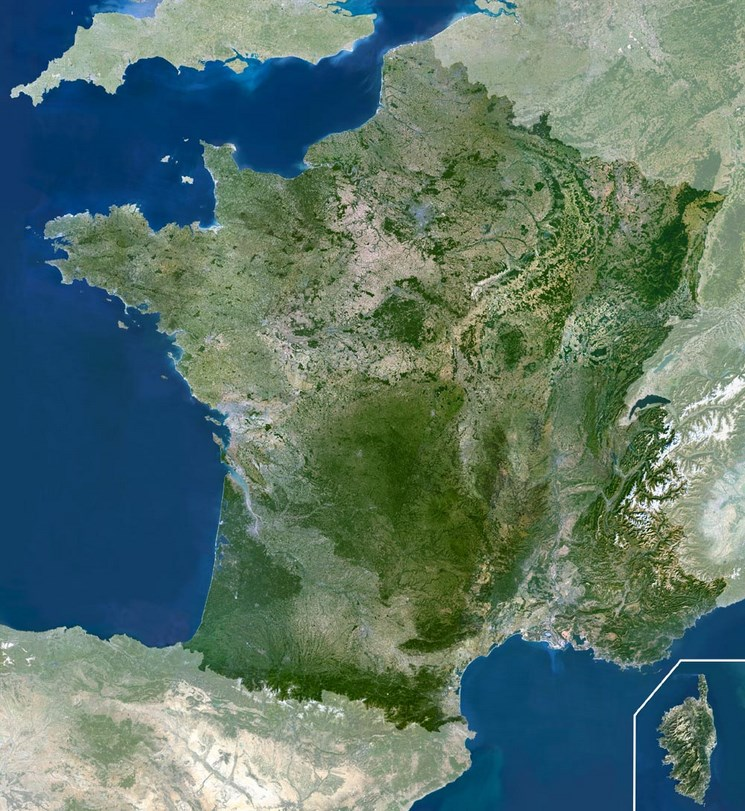
\includegraphics[scale=0.12]{figures/lib/france_satellite.jpg}};
    \node[align=center,below] at (photo.south) {Systeme modelise};
    % the local bounding box is to give a name to the pic:
    % http://tex.stackexchange.com/a/241737/32098
    \pic[local bounding box=carte] (carte) at (-5, 0) {france={scale 0.2}};
    \node[align=center,below] at (carte.south) {Modele};
    \draw[->] (carte) -- (photo.west) node[midway,above] {Represente} node[midway,below]{$\mu$};
\end{tikzpicture}

\end{center}
    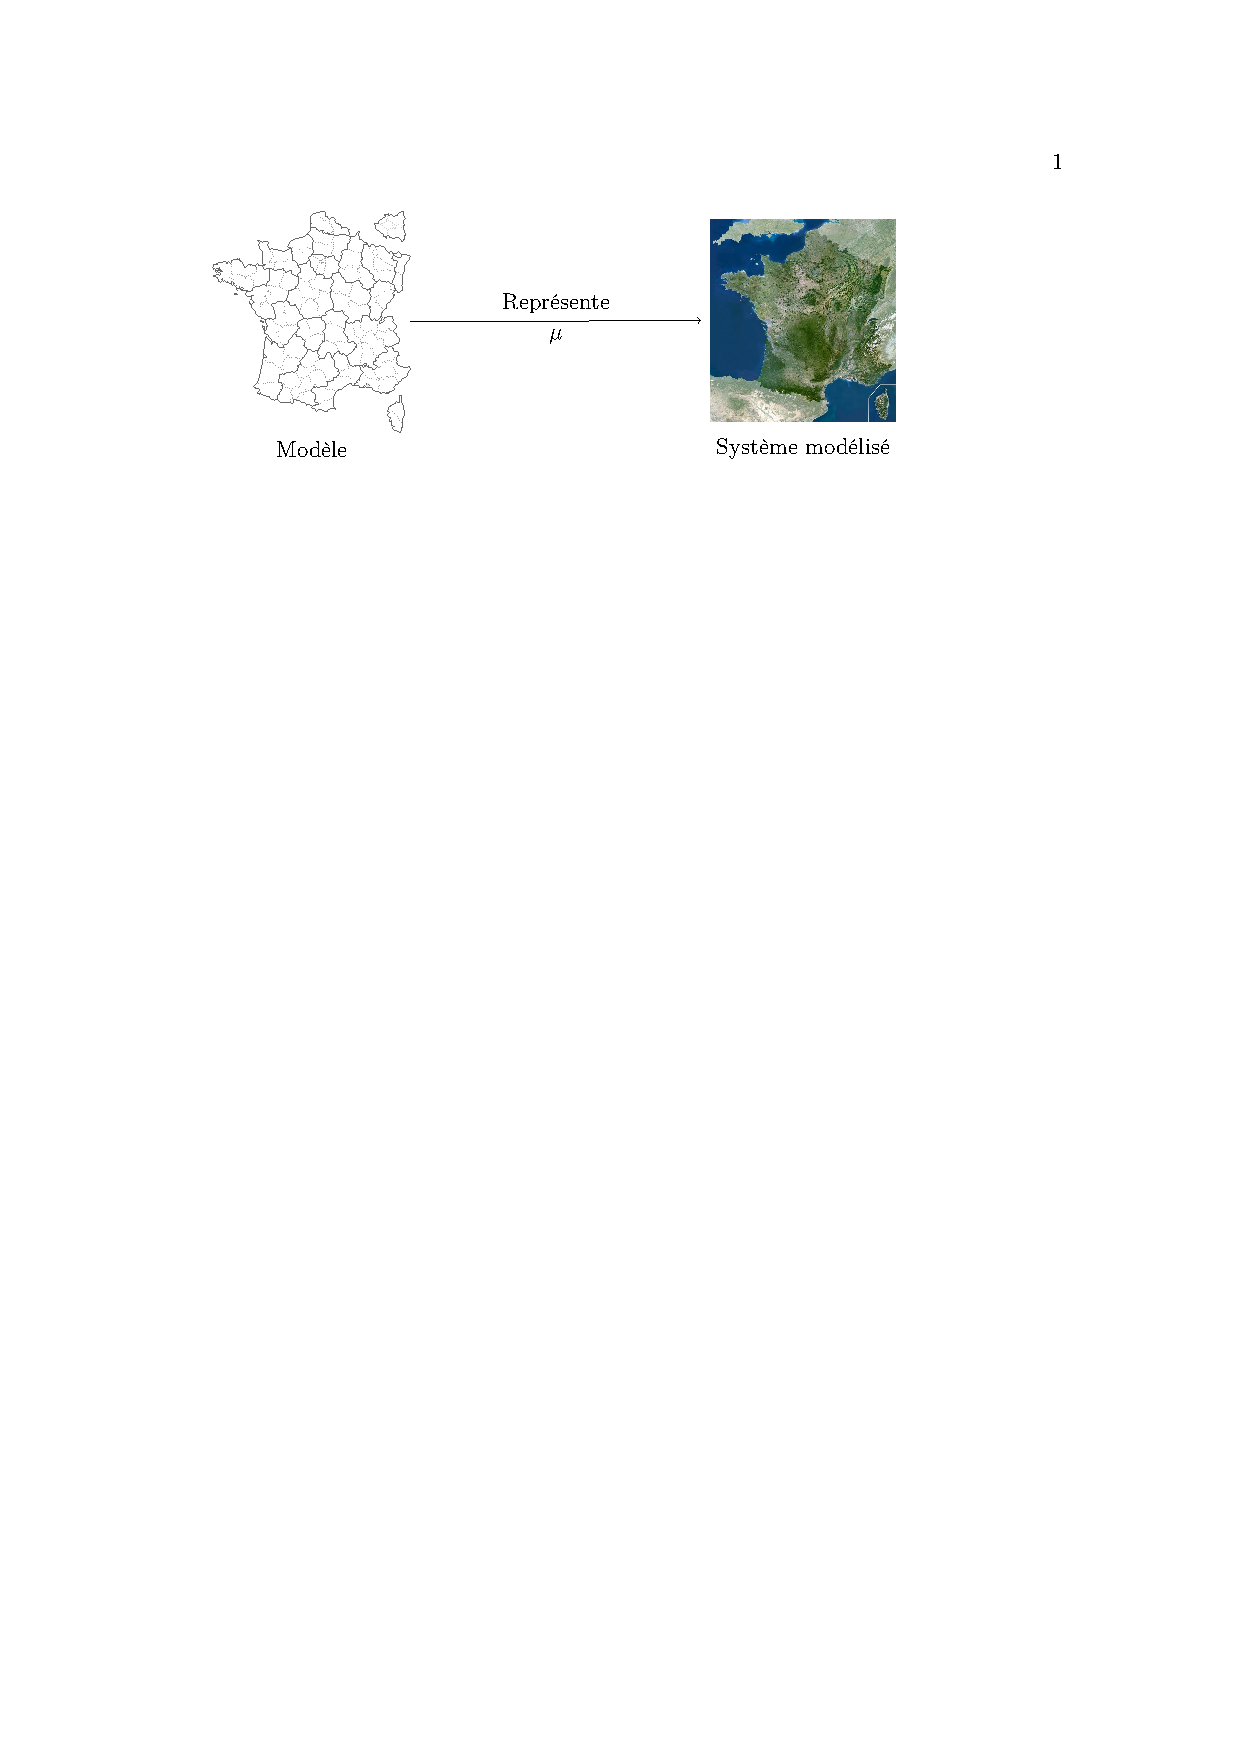
\includegraphics[trim= 100 635 400 100]{figures/3_etat_de_l_art_IDM/modele_france.pdf} %_BUILD_QUICK
    \caption{Relation entre système et modèle \protect\cite{favre2006ingenierie}}
    \label{fig:systemModele}
\end{figure}

Cette définition n'est pas restreinte à l'informatique et pourrait s'appliquer à 
n'importe quel système. 
La figure~\ref{fig:systemModele} reprend l'exemple connu de la cartographie où 
une carte géographique joue le rôle de modèle pour le territoire français qui joue le rôle su système réel.

L'intérêt de l'\gls{idm} est de produire des modèles exploitables informatiquement. 
Ceci n'est possible que si ces modèles sont décrits par des langages formels. Il 
devient alors important de bien définir ces langages à l'aide de métamodèles.

\subsection{Métamodèle et Conformité}
L'originalité de l'\gls{idm} ne réside pas dans la relation de représentation qui 
trouve plutôt son origine dans les méthodes de modélisation telles que Merise. L'apport de l'\gls{idm} est dans l'utilisation systématique de métamodèles pour la description des langages de modélisation. 

Il existe plusieurs définitions de la notion de métamodèle dans la littérature. 
Cependant la définition suivante est communément admise \cite{bezivin2004rapport}.
\\\

\begin{definition}
Un métamodèle est un modèle du langage de modélisation qui sert à exprimer les 
modèles.
\end{definition}

Une autre définition courante mais erronée de la notion de métamodèle suppose
qu'un métamodèle est un modèle de modèle. La figure~\ref{fig:modelofmodel}
reprend l'exemple de la cartographie évoquée plus haut. Nous appliquons
récursivement la relation \textit{Représente} $(\mu)$ au territoire français.
Ici, une carte de la France joue le rôle de modèle du territoire français. Un
fichier XML spécifiant l'éditeur, l'année d'édition et la langue de carte joue
le rôle de modèle de cette carte dans une base de données. Dans ce
contre-exemple, le fichier XML n'est pas un métamodèle de la carte administrative de la France
car il ne décrit pas les concepts utilisées par la carte et leurs relations. Un
métamodèle n'est donc pas un modèle d'un modèle.
% \hspace{-11cm}\raisebox{-5mm}[0pt][0pt]{%
% \makebox[0pt][l]{\parbox[t]{\linewidth}{\color{red}%
% Cet exemple n'est pas terrible. Le fichier XML peut être vu comme une sérialisation de la carte. Il vaudrait mieux considérer un modèle de la carte, qui en capture certaines informations pour une autre utilisation. Par exemple un modèle de la carte pour sa gestion dans une base de données : auteur, copyright, échelle, date de mise à jour, coordonnées géographiques de la zone représentée etc. On verrait alors mieux que ce modèle n'est pas un modèle du territoire, bien qu'il soit un modèle de la carte qui est un modèle du territoire.
% }}}

\begin{figure}[!ht]
    %_BUILD_FULL \begin{center}%\newsavebox\lstbox
%\begin{lrbox}{\lstbox}
%    \begin{minipage}{0.25\textwidth}
%        \begin{lstlisting}[style=xmlfig]
%<carte>
% <pays>France</pays>
% <regions>
%  <region>
%   <nom>Rhone-Alpes</nom>
%   <departement>
%    <nom>Drome</nom>
%   </departement>
%   ...
%  </region>
%  ...
% </regions>
%</carte>\end{lstlisting}
%    \end{minipage}
%\end{lrbox}

%\begin{tikzpicture}[]
%    \node (xml) at (-4, -1.86) {\usebox\lstbox};
%    \node[align=center,below] at (xml.south) {Modele};
%
%    % the local bounding box is to give a name to the pic:
%    % http://tex.stackexchange.com/a/241737/32098
%    \pic[local bounding box=carte] (carte) at (0, 0) {france={scale 0.2}};
%    \node[align=center,below] at (carte.south) {Modele};
%
%    \node[inner sep=4pt] (photo) at (7,-1.86) {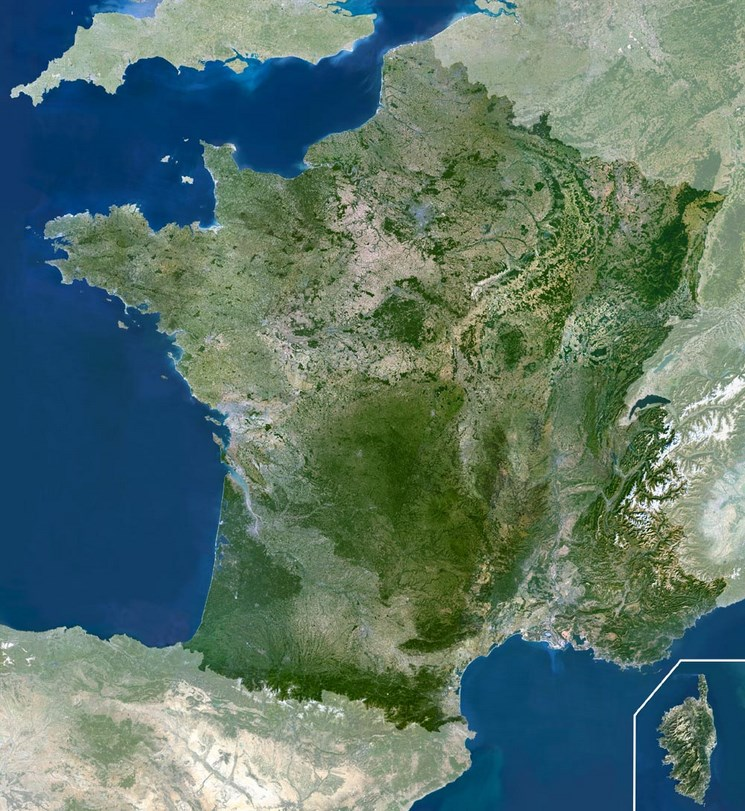
\includegraphics[scale=0.12]{figures/lib/france_satellite.jpg}};
%    \node[align=center,below] at (photo.south) {Systeme modelise};
%
%    \draw[->] (carte) -- (photo.west) node[midway,above] {Represente} node[midway,below]{$\mu$};
%    \draw[->] (xml) -- (carte.west) node[midway,above] {Represente} node[midway,below]{$\mu$};
%\end{tikzpicture}

\newsavebox\lstbox
\begin{lrbox}{\lstbox}
    \begin{minipage}{0.25\textwidth}
        \begin{lstlisting}[style=xmlfig]
<carte>
 <pays>France</pays>
 <region>
  <nom>Rhone-Alpes</nom>
  <departement>
   <nom>Drome</nom>
  </departement>
  ...
</carte>\end{lstlisting}
    \end{minipage}
\end{lrbox}
\begin{tikzpicture}[]
    \node (xml) at (-3.6, -1.4) {\usebox\lstbox};
    \node[align=center,below] at (xml.south) {Modele};

    % local bounding box to give a name to the pic: http://tex.stackexchange.com/a/241737/32098
    \pic[local bounding box=carte] (carte) at (0, 0) {france={scale 0.15}};
    \node[align=center,below] at (carte.south) {Modele};

    \node[inner sep=2pt] (photo) at (6,-1.4) {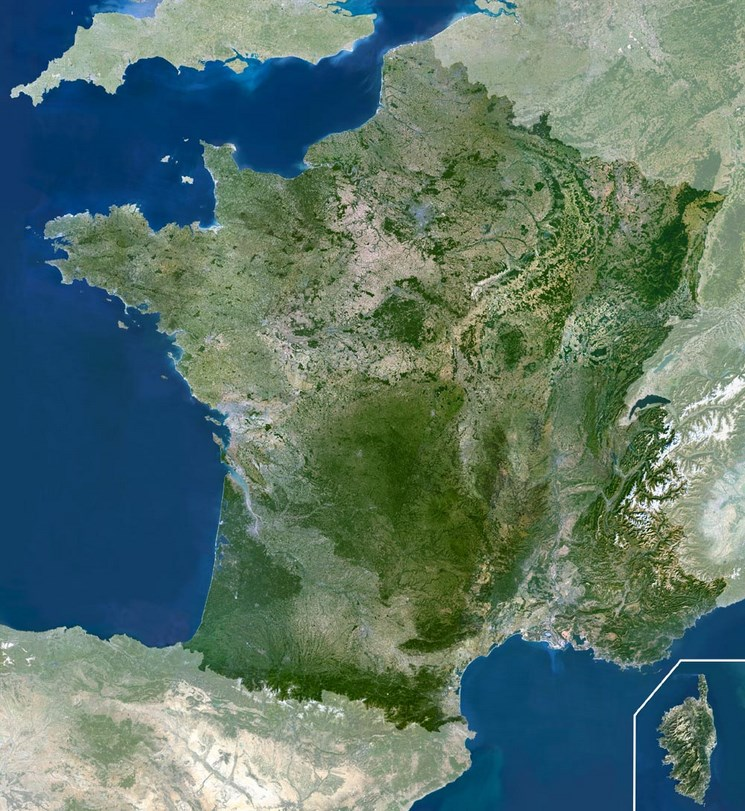
\includegraphics[scale=0.09]{figures/lib/france_satellite.jpg}};
    \node[align=center,below] at (photo.south) {Systeme modelise};

    % fleches
    \draw[->] (carte) -- (photo.west) node[midway,above] {Represente} node[midway,below]{$\mu$};
    \draw[->] (xml) -- (carte.west) node[midway,above] {Represente} node[midway,below]{$\mu$};
\end{tikzpicture}
\end{center}
    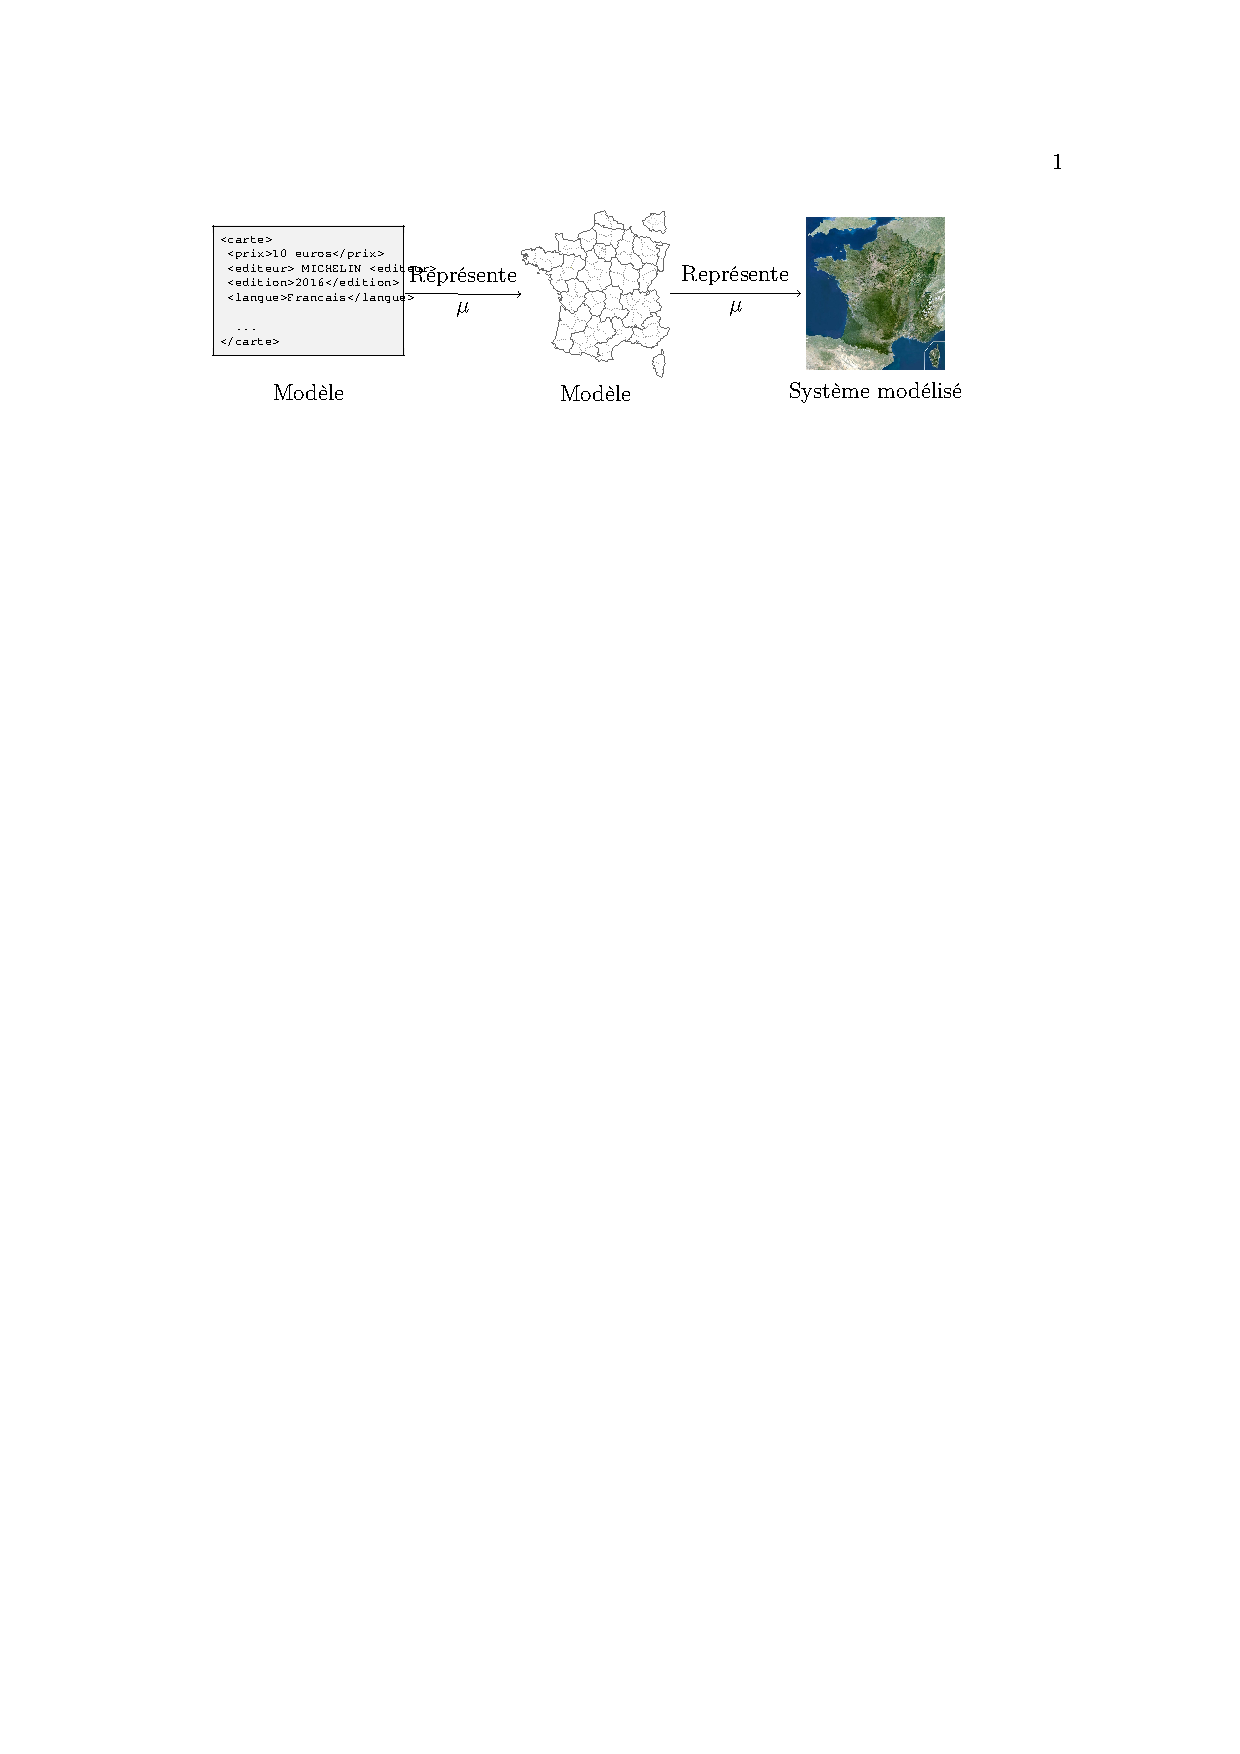
\includegraphics[trim= 100 635 400 100]{figures/3_etat_de_l_art_IDM/modele_carte.pdf} %_BUILD_QUICK
    \caption{Modèle de modèle selon l'exemple de la cartographie 
    \protect\cite{favre2006ingenierie}}
    \label{fig:modelofmodel}
\end{figure}

Par ailleurs, le concept de métamodèle induit la deuxième relation fondamentale 
de l'\gls{idm} liant un modèle à son métamodèle. Cette relation est nommée 
\textit{ConformeÀ} et notée $\chi$ \cite{bezivin2004search} 
\cite{favre2004towards}. La figure \ref{fig:carteFavre} reprend l'exemple de la 
cartographie. La légende de la carte peut être vue comme le métamodèle de la
carte de la France car elle spécifie les concepts utilisés pour modéliser la carte
(département et région) et leur relation (une région comporte des département).
Pour être lisible, la carte doit être conforme à la légende, c'est-à-dire utiliser
uniquement ces concepts. Cependant, la légende est un cas particulier de métamodèle 
qui définit la manière dont sont représentés les concepts. 

\begin{figure}[!ht]
    %_BUILD_FULL \begin{center}% http://tex.stackexchange.com/a/7816/32098
\begin{tikzpicture}[
    title/.style={font=\scriptsize},
    textlgd/.style={font=\tiny,inner sep=1pt}]

    \pic[local bounding box=carte] (carte) at (0, 0) {france={scale 0.15}};
    \node[align=center,below] (modele) at (carte.south) {Modèle};

    \begin{scope}[scale=0.7,xshift=-130,yshift=-60]
        \draw (-1.7cm,-1.7cm) rectangle (1.6cm,2.5cm);
        % HACK: \clip does not accept options such as line width, but we want a
        % thin line so we make this the default for this scope. Since we also
        % want to keep the default line width for the dotted line, we copy its
        % value in a length as showed here:
        % http://tex.stackexchange.com/a/65811/32098
        \newlength{\defaultpgflinewidth}
        \setlength{\defaultpgflinewidth}{\pgflinewidth}
        \begin{scope}[ultra thin]
            \clip[draw] (0,0) circle (1cm);
            \draw[densely dotted,line width=\defaultpgflinewidth,step=.5cm,gray] (-1.4,-1.4) grid (1.4,1.4);
        \end{scope}
        \node[textlgd] (dpt) at (105:1.7cm) {Departements};
        \node[textlgd] (reg) at (-120:1.7cm) {Region};
        \draw[->] (reg) -- (-120:1cm);
        \draw[->] (dpt) -- (0.25,0.25);
        \draw[->] (dpt) -- (-0.25,0.25);
        \node (legende) [title] at (0,2.2cm) { Légende };
    \end{scope}
    \path (modele) -- +(-4.5,0) node[align=center] {Métamodèle};

    \node[inner sep=2pt] (photo) at (6,-1.4) {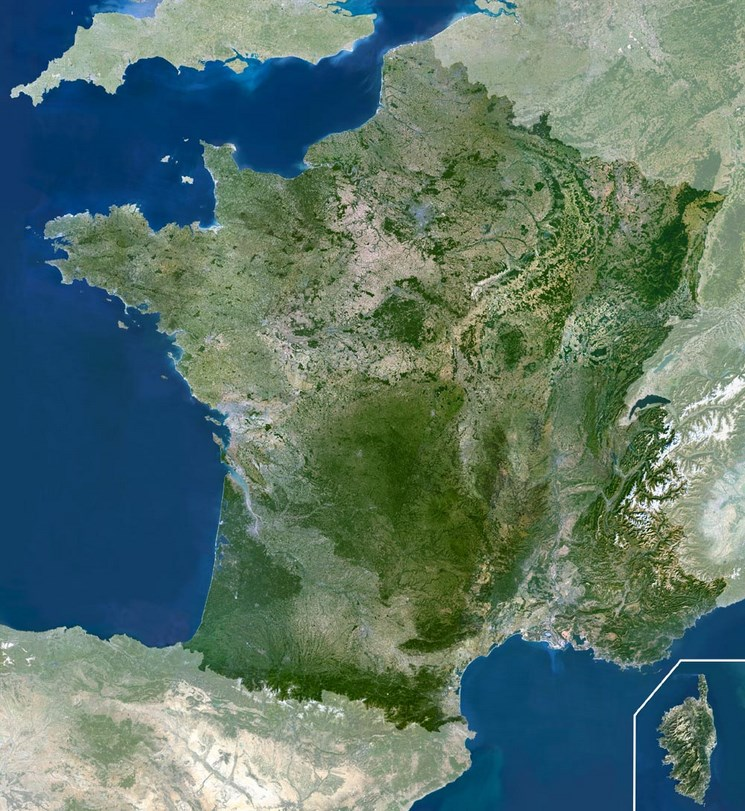
\includegraphics[scale=0.09]{figures/lib/france_satellite.jpg}};
    \path (modele) -- +(4.7,0) node[align=center] {Système modélisé};

   \draw[->] (carte) -- +(3.3,0) node[midway,above] {Représente} node[midway,below]{$\mu$};
   \draw[->] (carte) -- +(-3.2,0) node[midway,above] {ConformeÀ}  node[midway,below]{$\chi$};
\end{tikzpicture}
\end{center}
    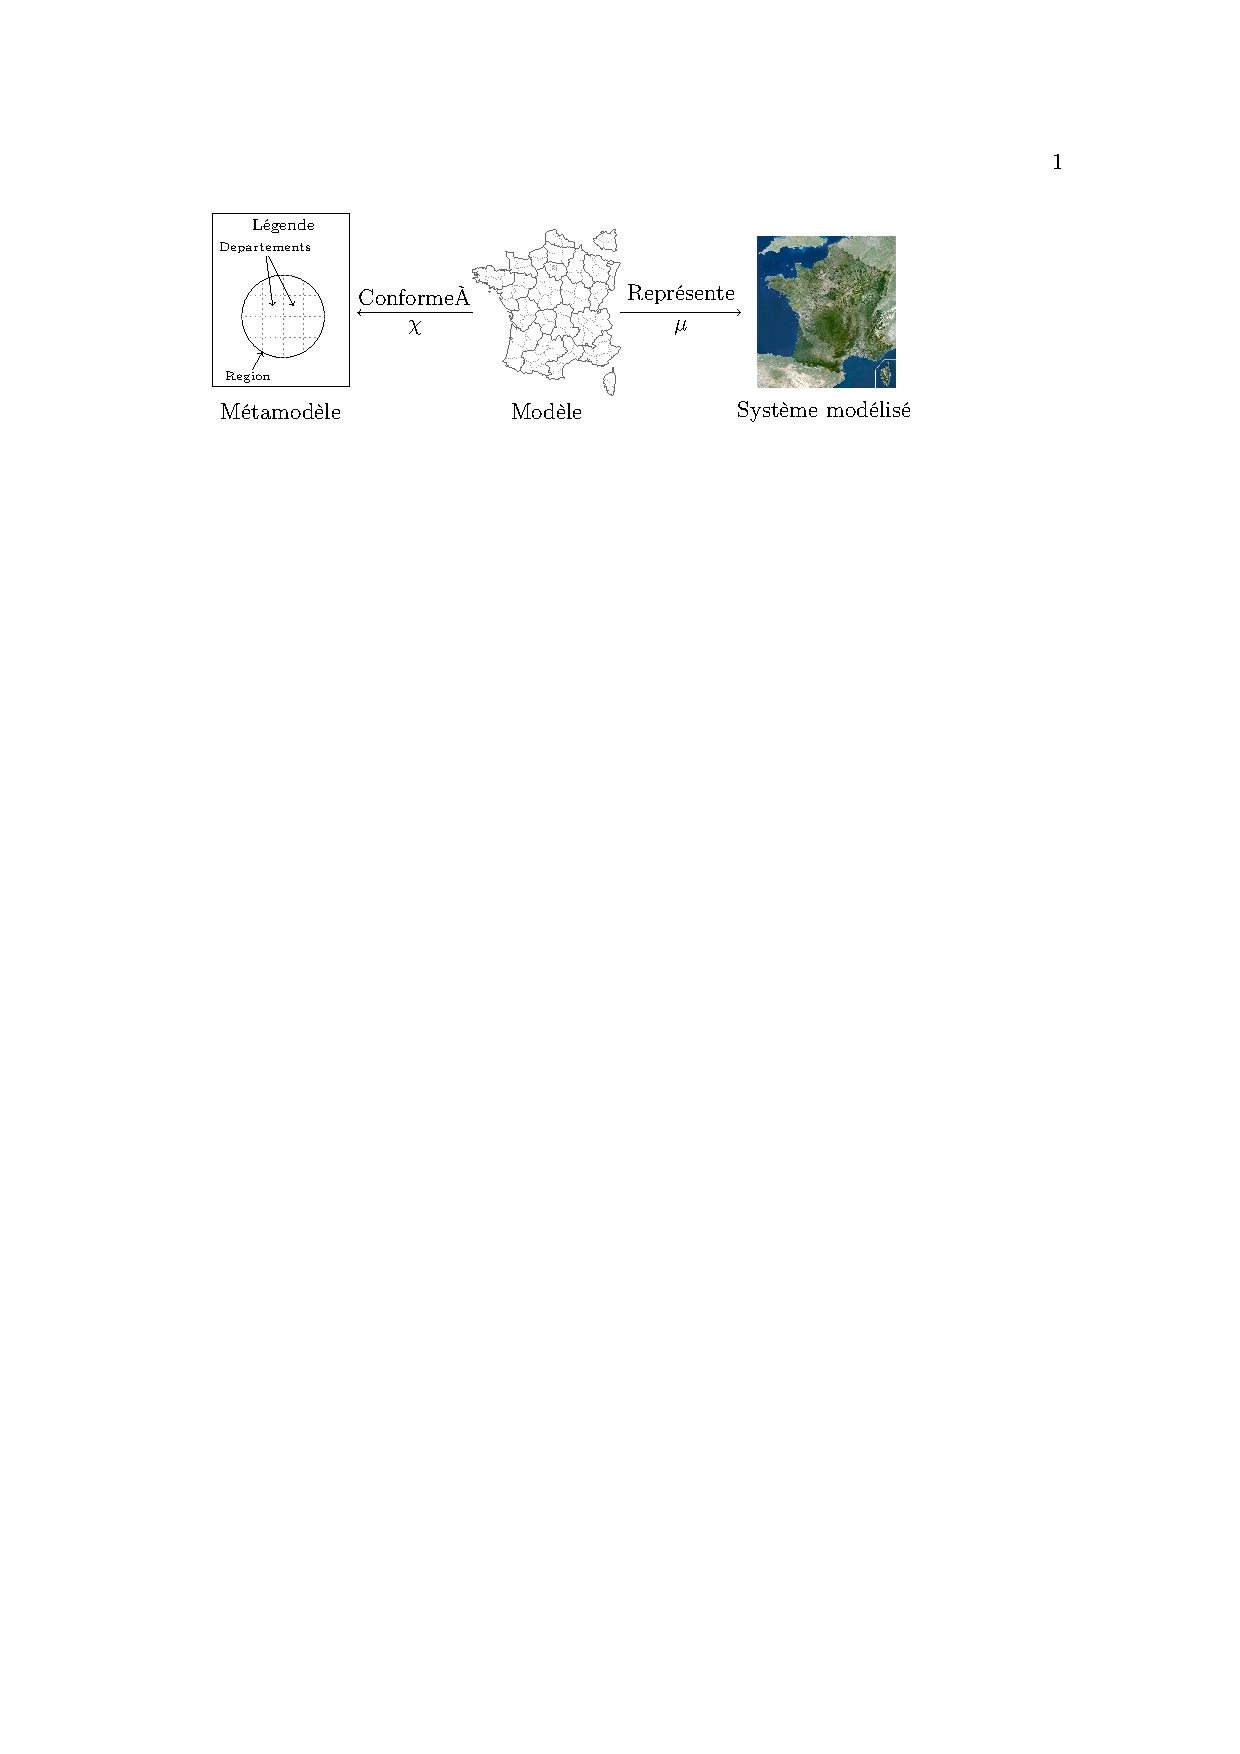
\includegraphics[trim= 100 635 400 100]{figures/3_etat_de_l_art_IDM/metamodel_carte.pdf} %_BUILD_QUICK
 \caption{Relations entre système, modèles, métamodèle et langage de 
modélisation \protect\cite{favre2006ingenierie}}
 \label{fig:carteFavre}
\end{figure}

% \raisebox{5mm}[0pt][0pt]{%
% \makebox[0pt][l]{\parbox[t]{\linewidth}{\color{red}%
% Cet exemple est faux. Une carte n'est pas conforme à sa légende.
% Il vaudrait mieux dire que si le modèle du territoire (la carte) est décrit en SVG, alors ce modèle est conforme au métamodèle de SVG. Tu dis toi-même qu'un métamodèle est un modèle d'un langage de modélisation. Le métamodèle de SVG est un modèle du langage SVG dans lequel la carte est décrite.
% }}}

\section{Transformation de modèle}
\label{sec:transfo_idm}
Comme expliqué précédemment, la préoccupation majeure de l'\gls{idm} est de 
rendre les modèles opérationnels sur tout le cycle de vie des systèmes 
logiciels, depuis l'analyse et la conception jusqu'à la maintenance et 
l'évolution. La transformation de modèle se retrouve au cœur de l'\gls{idm} car 
c'est à travers elle que se fait l'automatisation des traitements apportés aux 
modèles. Dans cette section, nous donnons une définition de la 
transformation de modèle avant d'en présenter les types et les usages.

\subsection{Définition de la transformation de modèle}
L'\gls{omg} définit une transformation de modèle comme «~le processus consistant à 
convertir un modèle en un autre modèle d'un même système~» \cite{omg2011meta}. 

Kleppe et al. \cite{kleppe2003mda} proposent une définition moins générique en insistant sur l'aspect automatique de ce processus~:~«~une transformation de modèle 
consiste en la génération automatique d'un modèle source en un modèle cible, 
selon une description établie de cette transformation~». Cette définition 
implique qu'une transformation est décrite à un niveau 
d'abstraction au dessus de celui des modèles~:~au niveau d'un métamodèle auquel elle doit se conformer. 

Mens et Van Gorp \cite{mens2006taxonomy} étendent cette définition en considérant qu'une 
transformation est une opération qui peut avoir en entrée un ou plusieurs 
modèles source et en sortie un ou plusieurs modèles cible~: 
\\\

\begin{definition}
Une transformation génère automatiquement un ou plusieurs modèles cible à partir 
d'un ou plusieurs modèles source, selon une description établie de la 
transformation. 
\end{definition}

C'est cette dernière définition que nous adoptons dans ce document. Par 
ailleurs, notons que, si les métamodèles source et cible sont différents, la 
transformation est dite exogène. Si les métamodèles source et cible 
sont identiques, la transformation est dite endogène. Ces 
termes sont introduits par Mens et Van Gorp \cite{mens2006taxonomy}.

\subsection{Composants d'une transformation de modèle} 
La figure \ref{fig:composantTransfo} illustre les composants d'une 
transformation de modèle~:~les modèles source, les modèles cible, la définition 
de la transformation et le moteur qui va effectuer la transformation selon sa 
définition. 

La description de la transformation définit la manière de transformer un ou plusieurs modèles source en un ou plusieurs modèles cible. Elle est créée dans 
un langage de transformation de modèle. Par exemple, si c'est un langage à base 
de règles, la description de la transformation consiste en un ensemble de règles 
de transformation à effectuer sur les modèles cible \cite{kleppe2003mda}. 

Un moteur de transformation exécute ou interprète la description. Il applique 
donc la description aux modèles source pour produire les modèles cible en 
suivant les étapes ci-dessous \cite{tratt2005model}~:

\begin{itemize}
\item identifier l'élément du ou des modèles source à transformer~;
\item pour chaque élément identifié, produire l'élément cible qui lui est 
associé dans le ou les modèles cible~;
\item produire une trace de la transformation qui lie les éléments du ou des 
modèles cibles aux éléments du ou des modèles source.
\end{itemize}

\begin{figure}[!ht]
    %_BUILD_FULL \begin{center}% http://tex.stackexchange.com/a/58828/32098
\newcommand{\gear}[3]{%
  \def\modu{#1}
  \def\Zb{#2}
  \def\AngleA{#3}

  \pgfmathsetmacro{\Rpr}{\Zb*\modu/2}
  \pgfmathsetmacro{\Rb}{\Rpr*cos(\AngleA)}
  \pgfmathsetmacro{\Rt}{\Rpr+\modu}
  \pgfmathsetmacro{\Rp}{\Rpr-1.25*\modu}
  \pgfmathsetmacro{\AngleT}{pi/180*acos(\Rb/\Rt)}
  \pgfmathsetmacro{\AnglePr}{pi/180*acos(\Rb/\Rpr)}
  \pgfmathsetmacro{\demiAngle}{180/\Zb}
  \pgfmathsetmacro{\Angledecal}{(\demiAngle-2*\AnglePr)/2}

  \foreach \zz in{1,2,...,\Zb}{
    \draw
    ({(\zz))/\Zb*360-\Angledecal}:\Rb)
    -- (\zz/\Zb*360-\Angledecal:\Rp)
    to[bend right=\demiAngle]
    (\zz/\Zb*360+\Angledecal:\Rp)
    --
    plot[domain=-0:\AngleT,smooth,variable=\t]
    ({{180/pi*(-\t+tan(180/pi*\t)) +\zz/\Zb*360+\Angledecal}:\Rb/cos(180/pi*\t)})
    % 
    to[bend right=\demiAngle]
    ({{180/pi*(\AngleT+tan(180/pi*-\AngleT)) +(\zz+1)/\Zb*360-\Angledecal}:
      \Rb/cos(180/pi*-\AngleT)})
    % 
    plot[domain=-\AngleT:-0,smooth,variable=\t]
    ({{180/pi*(-\t+tan(180/pi*\t)) +(\zz+1)/\Zb*360-\Angledecal}:\Rb/cos(180/pi*\t)});
  }
}

\begin{tikzpicture}

    \begin{scope}[xshift=-3.3cm,yshift=0.5cm]
        \node [densely dotted,minimum height=1cm,fill=gray!75!white,opacity=0.8,minimum width=2cm,draw,rectangle,rounded corners=3pt] {};
        \node [xshift=0.1cm,yshift=-0.1cm,densely dotted,minimum height=1cm,fill=gray!25!white,opacity=0.7,minimum width=2cm,draw,rectangle,rounded corners=3pt] {};
        \node [xshift=0.2cm,yshift=-0.2cm,minimum height=1cm,minimum width=2cm,draw,fill=white,opacity=0.8,rectangle,rounded corners=3pt,font=\footnotesize,align=center] (left) {modeles\\ source};
        \draw[->] (left) -- (2.5cm,-0.2cm);
    \end{scope}
    \begin{scope}[xshift=6.6cm,yshift=0.5cm]
        \node [densely dotted,minimum height=1cm,fill=gray!75!white,opacity=0.8,minimum width=2cm,draw,rectangle,rounded corners=3pt] {};
        \node [xshift=0.1cm,yshift=-0.1cm,densely dotted,minimum height=1cm,fill=gray!25!white,opacity=0.7,minimum width=2cm,draw,rectangle,rounded corners=3pt] {};
        \node [xshift=0.2cm,yshift=-0.2cm,minimum height=1cm,minimum width=2cm,draw,fill=white,opacity=0.8,rectangle,rounded corners=3pt,font=\footnotesize,align=center] (right) {modeles\\ cibles};
    \draw[<-] (right) -- (-2.1cm,-0.2cm);
    \end{scope}
    \draw (-0.8,-1.1) rectangle (4.5,1.7);
    \begin{scope}[scale=1]
        % fichier (http://tex.stackexchange.com/a/174673/32098)
        \draw (0,0) -- (0,1.2) -- (0.7,1.2) -- (0.7,0.8) -- (1,0.8) -- (1,0) -- cycle;
        \draw (0.7,1.2) -- (1,0.8);
        \foreach \y in {0.2,0.4,0.6}{
            \draw (0.2,\y) -- (0.8,\y);
            \draw (0.2,0.8) -- (0.6,0.8);
            \draw (0.2,1) -- (0.6,1);
        }
        \node at (0.4,-0.6) [rectangle,align=center,font=\scriptsize] {Definition de\\ la transformation};
        \node at (1.8,0.5) {$+$};
        \begin{scope}[xshift=3.2cm,yshift=0.8cm,rotate=-60]
            \begin{scope}[scale=0.02]
                \gear{3}{15}{20}
                \begin{scope}[xshift=40.5cm,rotate=180/12]
                    \gear{3}{12}{20}
                \end{scope}
            \end{scope}
        \end{scope}
        \node at (3.3,-0.6) [rectangle,align=center,font=\scriptsize] {Engin de\\ la transformation};
    \end{scope}

\end{tikzpicture}
\end{center}
    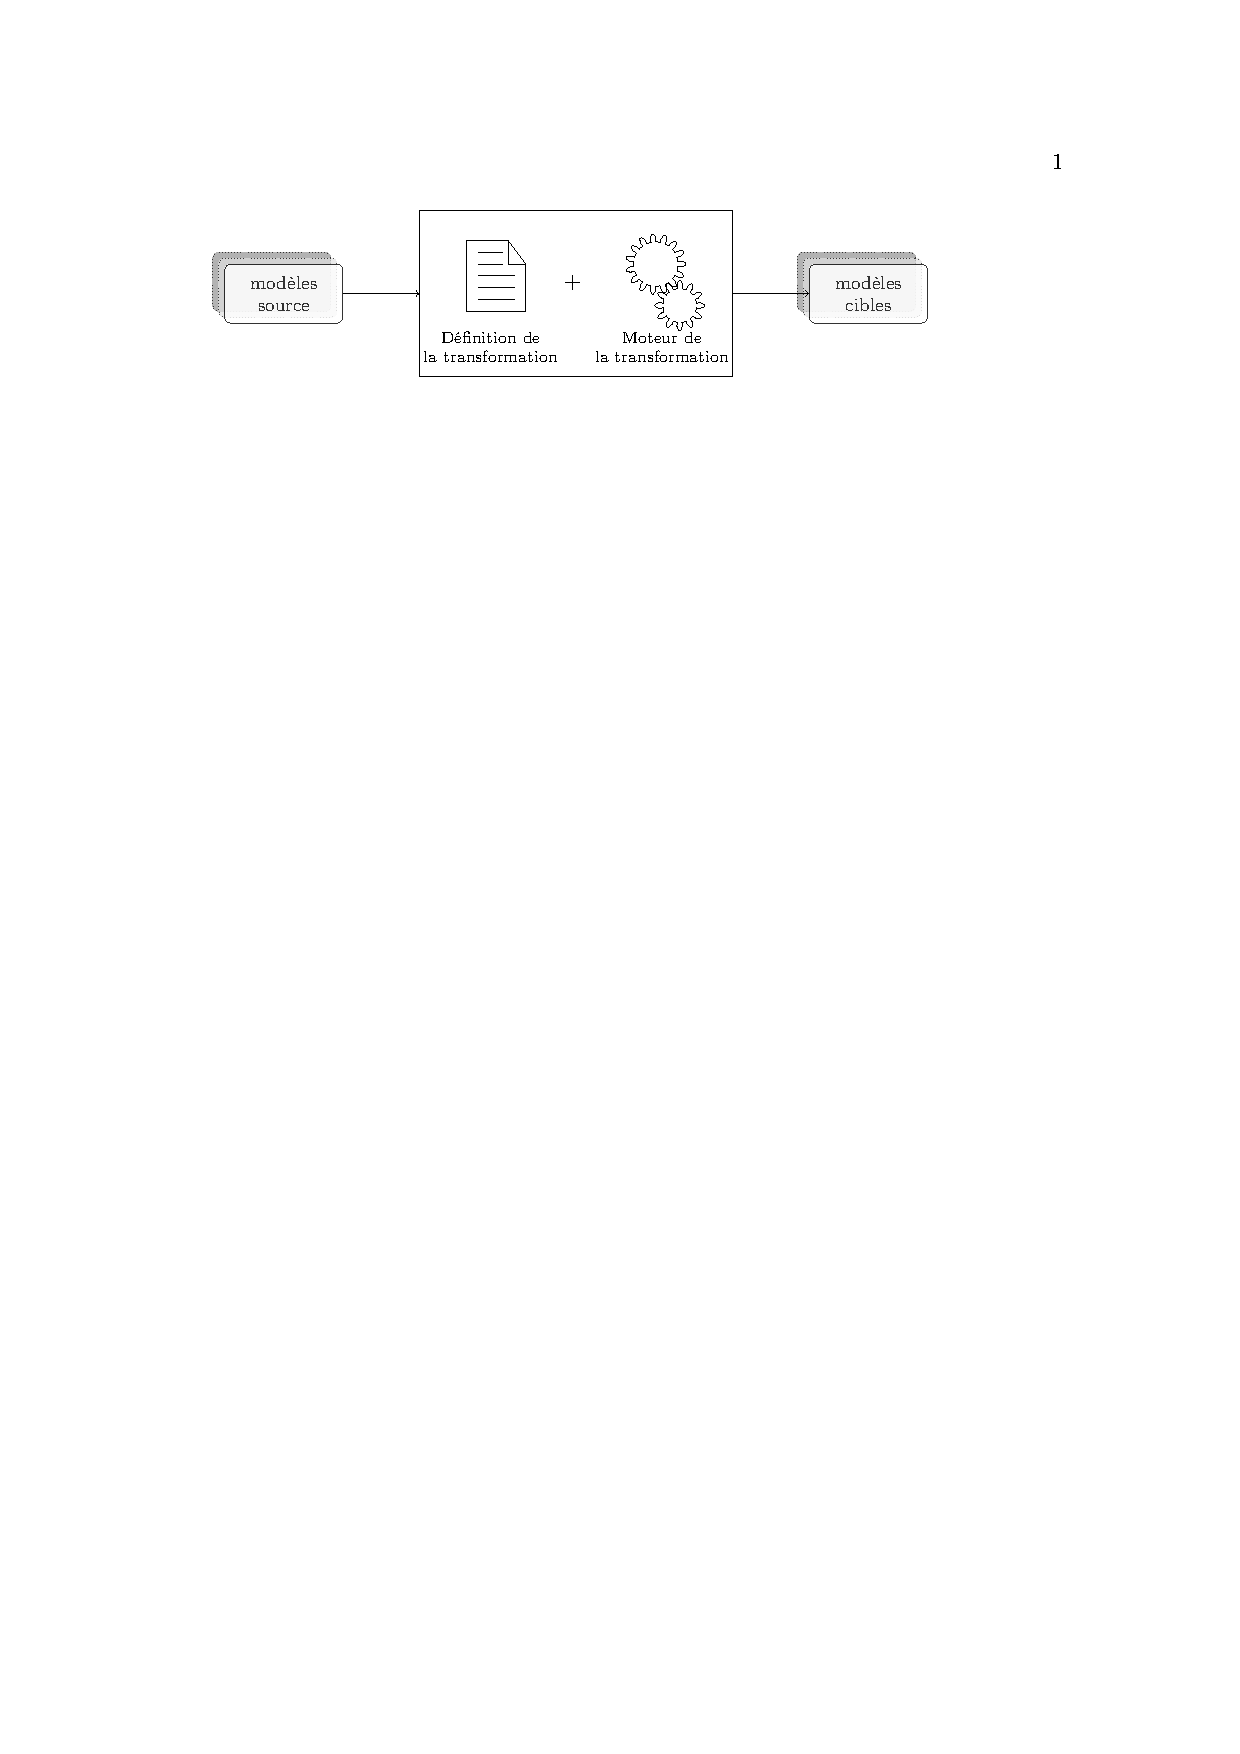
\includegraphics[trim= 100 635 400 100]{figures/3_etat_de_l_art_IDM/composants_transfo.pdf} %_BUILD_QUICK
    \caption{Composants d'une transformation de modèle}
    \label{fig:composantTransfo}
\end{figure}

\subsection{Usages de la transformation de modèles }
Les transformations de modèles sont au cœur d'une démarche dirigée par les 
modèles~:~elles permettent d'automatiser les manipulations subies par les 
modèles telles que la modification, la création, l'adaptation, la composition ou 
encore le filtrage de modèles, à travers la réutilisation systématique 
d'informations contenues dans les modèles existants. 

Il est possible de recourir aux transformations de modèles sur tout le cycle de 
vie d'un système. Les usages les plus répandus sont le raffinement, 
l'intégration d'outils, la composition, l'analyse, la simulation et 
l'optimisation que nous présentons dans la suite de ce document. 


\subsubsection{Raffinement}

Le raffinement consiste à rajouter plus de détails au modèle initial. Ce type de 
transformation peut aussi bien être endogène (métamodèles source et cible 
identiques) ou exogène (métamodèle source et cible différents). Le raffinement se 
prête parfaitement à toute la partie descendante du cycle en V où les modèles 
passent à des niveaux d'abstraction plus bas. Ceci revient à faire des 
transformations successives de type modèle-à-modèle et une transformation de 
type modèle-à-texte pour aboutir au code final.

Raffiner un modèle revient à décomposer des concepts de haut niveau, à choisir 
un algorithme particulier, à spécialiser un concept pour un contexte donné ou 
encore à le concrétiser sous forme d'une solution exécutable par une machine en 
générant le code à partir de modèles de plus haut niveau d'abstraction 
\cite{czarnecki2000intentional}. 

\subsubsection{Intégration d'outil}

Il existe une panoplie d'outils disponibles pour créer, manipuler, analyser ou 
encore simuler des modèles. Souvent ces outils utilisent des métamodèles 
internes et des espaces techniques qui leurs sont propres. Ainsi, l'échange de 
modèles entre ces outils est compromis et l'interopérabilité est fortement 
entravée. L'utilisateur se trouve obligé d'utiliser un seul et même outil sur 
tout le cycle de vie du système et ne peut donc pas tirer avantage des 
possibilités offertes par d'autres outils plus adaptés à ses besoins à certaines 
étapes.

L'intégration d'outil est une solution pour pallier la divergence syntaxique et 
sémantique des outils et des langages de modélisation par le biais la 
transformation de modèle \cite{tratt2005model}. Ce type de transformation permet 
de naviguer entre deux métamodèles, de synchroniser des modèles qui évoluent 
séparément sur des outils distincts, d'établir des correspondances entre métamodèles pour 
maintenir la cohérence des modèles conformes à ces métamodèles. Il sera donc 
possible de faire appel à des outils mieux adaptés à chaque étape du cycle de 
vie.

\subsubsection{Composition}

Pour réduire la complexité inhérente à la modélisation et à l'analyse de grands 
systèmes, tels que les Smart Grids par exemple, il est possible d'adopter une 
approche par points de vue qui permet de séparer les préoccupations. Les modèles 
produits correspondent donc à ces différents points de vue qu'on peut ainsi 
valider séparément dans un premier temps. A l'issue de cette approche modulaire, 
on pourra composer ces modèles, c'est-à-dire les assembler, pour aboutir un 
modèle global du système.

Dans le cas le plus simple, les deux modèles à composer sont conformes à un même 
métamodèle. Cependant, il est aussi possible de composer deux modèles conformes 
à deux métamodèles différents. 

Les deux modèles à composer peuvent aussi présenter des concepts en commun. Deux 
techniques existent pour composer des modèles~:
%que nous illustrons dans la figure \ref{fig:compoExemple}~:

\begin{itemize}
\item la première technique consiste à les fusionner. Dans ce cas, le modèle 
final résultant de la composition doit contenir toutes les informations issues 
des modèles initiaux, sans duplication des informations communes 
\cite{bezivin2006canonical}.
\cite{fleurey2008generic} présente un framework générique capable de composer 
des modèles indépendamment de leurs langages de modélisation. L'approche 
consiste à identifier les éléments qui représentent le même concept dans les 
deux modèles à composer et à les fusionner dans un nouveau modèle qui représente 
une vue intégrée de ces concepts. Il est aussi possible de spécialiser le 
framework pour un métamodèle particulier mais qui reste conforme au \gls{mof}~;

\item la deuxième technique consiste à les tisser. Dans ce cas, on crée des 
correspondances entre les éléments qui représentent un même concept. Un 
métamodèle générique est créé pour définir les correspondances qui sont donc 
modélisées dans le modèle final. On y retrouve donc les éléments en commun 
dupliqués mais liés par un lien de correspondance. 
\end{itemize}

Il est à noter que le modèle issu du tissage de deux modèles $M_{A}$ et $M_{B}$ 
peut être utilisé comme modèle intermédiaire que l'on note $M_{T}$ pour la 
fusion de $M_{A}$ et $M_{B}$. Dans ce cas, l'opération de fusion consiste à 
produire un modèle $M_{AB}$ en prenant comme entrée $M_{A}$, $M_{B}$ et $M_{T}$. 
Cette technique est notamment utilisée par \cite{del2007semi} pour la 
composition semi-automatique de modèles.

%\begin{figure}[!ht]
% \begin{center}
%  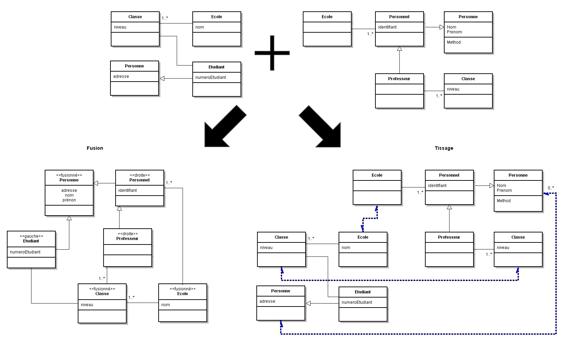
\includegraphics[width=1\textwidth]{figures/images/Chapitre1/compoExemple.png}
% \end{center}
% \caption{Exemple de composition de deux modèles}
% \label{fig:compoExemple}
%\end{figure}

\subsubsection{Simulation}

La transformation de modèle peut être utilisée pour simuler des modèles. En 
effet, une transformation de modèle peut mettre à jour le système modélisé. Dans 
ce cas, le modèle cible est une mise à jour du modèle source et la 
transformation est de type sur-place (modèles source et cible confondus). 

Par exemple, \cite{syriani2011multi} simule un comportement simple d'un jeu de 
Pacman en utilisant la transformation de modèle. La transformation spécifie les 
règles de transition qu'une instance du jeu peut prendre (Pacman et fantôme se 
trouvant dans la même case, Pacman et pomme se trouvant dans la même case, 
etc.). En ingénierie des langages, ceci revient à définir la sémantique 
opérationnelle d'un langage de modélisation. L'exécution de la transformation 
anime le modèle en fonction du comportement qu'on lui confère.

La transformation peut aussi être utilisée comme intermédiaire dans la 
simulation de modèle. Des modèles en entrée d'un outil de simulation externe 
sont produits par une transformation des modèles que l'on souhaite simuler. Cette 
technique permet de tirer profit d'outils de simulation existant sur le marché 
en utilisant l'intégration d'outils.

\subsubsection{Analyse et optimisation}

La transformation de modèle peut être utilisée pour les activités d'analyse de 
modèle. Une analyse simple telle que le calcul de métrique de similarité entre 
deux modèles via la transformation de modèle est donnée dans \cite{del2007semi} 
avec un modèle de transformation écrit en \gls{atl} \cite{jouault2006transforming}. 

Des analyses plus complexes sont possibles grâce à l'intégration d'outils 
d'analyse externes vers lesquels les modèles source sont transformés.

\cite{biehl2010integrating} propose d'utiliser la transformation de modèle pour 
l'analyse de sûreté de fonctionnement dans le domaine de l'automobile. Les 
modèles source sont transformés en modèles conformes au métamodèle de l'outil 
d'analyse de sûreté de fonctionnement retenu.
 
L'optimisation vise à améliorer les propriétés non fonctionnelles des modèles 
telle que l'évolutivité, la fiabilité, la modularité, etc. L'optimisation est 
typiquement utilisée sur les modèles d'architecture. Les transformations 
utilisées pour l'optimisation sont de types endogène car on cherche à affiner 
la conception de modèles existants. La réingénierie est un exemple de 
transformation utilisée pour optimiser les modèles en cherchant à améliorer la 
maintenabilité, la lisibilité et l'évolutivité des modèles.


\subsection{Approches existantes pour la transformation de modèle}  
Le recours à la transformation de modèle est l'objet de recherches informatiques 
antérieures à l'apparition de l'approche \gls{idm}. Par exemple, les compilateurs 
utilisent la transformation pour passer du code source au fichier binaire 
\cite{aho1985compilers}. Même si ce type de transformation trouve son origine dans le domaine de 
la programmation informatique, la transformation de modèle embrasse un champ d'application 
plus large encore.

Nous trouvons dans la littérature plus d'une trentaine d'approches différentes 
de transformation de modèle \cite{syriani2011multi}. Czarnecki et Helsen 
proposent une classification de ces approches selon plusieurs critères tels que 
le paradigme retenu pour définir la transformation, la relation entre les 
modèles sources et cibles, la directivité de la transformation, le nombre de 
modèles cible et source, l'orchestration et l'ordonnancement des règles de 
transformation, etc. \cite{czarnecki2006feature}. \cite{blanc2011mda} définit les trois grandes catégories d'approches suivantes.

\begin{description}

\item[Par programmation]:~Les modèles offrent une interface qui permet d'écrire les transformations dans 
un langage de programmation. Mais cette technique relève plus de la 
programmation que de la modélisation. Ce sont en fait des applications 
informatiques qui ont la particularité de manipuler des modèles. L'avantage de 
cette approche est qu'elle utilise un langage de programmation généraliste tel 
que Java ou C++ pour écrire les transformations. Ainsi le programmeur n'a pas 
besoin d'apprendre un nouveau langage. Cependant ces applications ont tendance à 
devenir difficilement maintenables.

\item [Par template]:~Dans cette approche, des canevas des modèles cible sont définis. Ces modèles contiennent des paramètres qui sont remplacés par les informations contenues 
dans les modèles source. Ce type de transformation est souvent utilisé pour les 
transformations qui génèrent des modèles dont la syntaxe concrète est textuelle.  Cette approche est associée au patron de conception \textit{visitor} qui va traverser la structure interne du modèle source. 
%Cette approche est utilisée par l'outil Enterprise Architect par exemple. 

\item [Par modélisation]:~Cette approche vise à appliquer les principes de l'\gls{idm} aux transformations de modèle elles-mêmes. Les modèles de transformation sont ainsi pérennes, réutilisables et indépendants des plates-formes d'exécution  \cite{bezivin2006model}. Pour cela, des langages de modélisation dédiés à l'activité de transformation de modèle sont utilisés. Cette approche considère donc la transformation comme 
un modèle à part entière conforme à un métamodèle de transformation. La figure 
\ref{fig:TransfoPrincipe} illustre cette approche en positionnant la transformation par rapport aux niveaux d'abstraction de l'\gls{idm}. Elle corrobore 
ainsi la vision unificatrice de l'\gls{idm} à travers le paradigme du «~tout est 
modèle~»\cite{bezivin2005unification}.
\end{description}


\begin{figure}[!ht]
 \begin{center}
  \begin{tikzpicture}[
    mynode/.style={inner sep=0pt,rectangle,draw,font=\footnotesize,align=center,minimum height=1.2cm,minimum width=3cm},
    legende/.style={midway,fill=white,font=\scriptsize}]
    \foreach \i in {1,...,3} {
        \foreach \j in {3,...,1} {
            \ifthenelse{\i=1}{
                \ifthenelse{\j=1}{\def\mytext{Meta-modele A}}{}
                \ifthenelse{\j=2}{\def\mytext{Modele A}}{}
                \ifthenelse{\j=3}{\def\mytext{Monde reel\\ Objet A}}{}
            }{}
            \ifthenelse{\i=2}{
                \ifthenelse{\j=1}{\def\mytext{Meta-modele de\\ la transformation}}{}
                \ifthenelse{\j=2}{\def\mytext{Description de\\ la transformation}}{}
                \ifthenelse{\j=3}{\def\mytext{Execution de\\ la transformation}}{}
            }{}
            \ifthenelse{\i=3}{
                \ifthenelse{\j=1}{\def\mytext{Meta-modele B}}{}
                \ifthenelse{\j=2}{\def\mytext{Modele B}}{}
                \ifthenelse{\j=3}{\def\mytext{Monde reel\\ Objet B}}{}
            }{}
            \node at (5*\i,-3*\j) [mynode] (\i\j) {\mytext} ;
        }
    }
    \node at (10,0) [mynode] (top) {meta-meta-modele};

    \draw[-angle 60] (11) -- (top) node [style=legende] {conformeA};
    \draw[-angle 60] (21) -- (top) node [style=legende] {conformeA};
    \draw[-angle 60] (31) -- (top) node [style=legende] {conformeA};

    \draw[-angle 60] (12) -- (11) node [style=legende] {conformeA};
    \draw[-angle 60] (12) -- (13) node [style=legende] {represente};

    \draw[-angle 60] (22) -- (21) node [style=legende] {conformeA};
    \draw[-angle 60] (22) -- (23) node [style=legende] {represente};

    \draw[-angle 60] (32) -- (31) node [style=legende] {conformeA};
    \draw[-angle 60] (32) -- (33) node [style=legende] {represente};

    \draw[-angle 60,densely dotted] (22) -- (11) node [style=legende] {se refere a};
    \draw[-angle 60,densely dotted] (22) -- (31) node [style=legende] {se refere a};
    \draw[-angle 60,densely dotted] (23) -- (12) node [style=legende] {se refere a};
    \draw[-angle 60,densely dotted] (23) -- (32) node [style=legende] {se refere a};
\end{tikzpicture}

 \end{center}
 \caption{Méta niveaux d'une transformation de modèle}
 \label{fig:TransfoPrincipe}
\end{figure}


	\subsection{Langages et outils pour la transformation de modèle}
Sans viser l'exhaustivité, nous introduisons succinctement quelques langages et outils 
dédiés à la transformation de modèles.  

\subsubsection{ATL}
\label{sec:ATL}
\gls{atl}\footnote{http://www.eclipse.org/atl/} est né de la volonté de proposer des langages de modélisation dédiés à la transformation de modèle en définissant un métamodèle 
et des outils pour l'exécution des transformations. 
%Il permet de réaliser des transformations de type modèle-à-modèle et de type modèle-à-texte.

\gls{atl} est un langage hybride (déclaratif et impératif) à base de contraintes \gls{ocl} \cite{jouault2006transforming}. 
%Une règle déclarative, appelée \textit{Matched rule}, permet de décrire 
%l'implémentation de mapping simples entre les modèles source et cible en 
%utilisant des patrons source (\textit{InPattern}) mappés avec les éléments 
%source et des patrons cibles (\textit{OutPattern}) mappés avec les éléments 
%cible. 

%L'approche impérative explicite les étapes d'exécution de la transformation à 
%travers les \textit{Helpers}. Le mécanisme de \textit{Helpers} permet en outre d'éviter la 
%redondance de code et la création de longues règles écrites en \gls{ocl}, ce qui 
%confère une meilleure lisibilité aux programmes \gls{atl}. 
%
%Une transformation écrite en \gls{atl} est composée d'un ensemble de règles qui 
%spécifient comment créer et initialiser les éléments des modèles cible. Il n'est 
%pas possible de spécifier l'ordre d'exécution des règles de transformation. Cet 
%ordre est établi automatiquement, sauf  pour les \textit{Lazy rules} 
%qui demandent de faire spécifiquement appel à elles. \gls{atl} est conforme au 
%méta-métamodèle \gls{mof} et est doté d'une syntaxe concrète textuelle. Il est intégré 
%à l'environnement Eclipse. Une transformation prend en entrée un ensemble de 
%modèles conformes au méta-métamodèle Ecore ou à KM3 \cite{jouault2006km3}.

%\gls{atl} ne prend pas en charge les transformations incrémentales. Il commence par 
%lire entièrement les modèles source et génère des modèles cible complet. Les 
%modifications manuelles dans les modèles cible ne sont donc pas préservées si 
%l'on opère une nouvelle transformation.

\gls{atl} peut réaliser des transformations sur place, c'est-à-dire, une 
transformation où le modèle source et le modèle cible sont confondus en 
utilisant le mode raffinement de modèle. 

%Cependant ce mode présente quelques limitations avec certaines fonctionnalités comme celle des \textit{Lazy rules}.

\subsubsection{QVT}
\gls{qvt} \cite{kurtev2008state} \cite{omg2011meta} est un standard de l'\gls{omg}. Le métamodèle de \gls{qvt} est conforme au \gls{mof}. Comme \gls{atl}, \gls{qvt} se base sur \gls{ocl} pour accéder aux éléments des modèles.
\gls{qvt} définit deux langages de transformation de type modèle-à-modèle. 
QVT \textit{Declarative} (QVTd)\footnote{http://projects.eclipse.org/projects/modeling.mmt.qvtd} est un langage déclaratif. QVT \textit{Operational} (QVTo) est un langage impératif\footnote{http://projects.eclipse.org/projects/modeling.mmt.qvt-oml}.

%QVT-R est un langage de transformation de haut niveau d'abstraction doté de 
%syntaxes concrètes textuelle et graphique. Les transformations, 
%bidirectionnelles, sont spécifiées sous forme de relations entre les modèles 
%source et cible. Une transformation a pour but de vérifier la cohérence entre 
%deux modèles, renforcer la cohérence en modifiant le modèle cible, synchroniser 
%deux modèles ou encore pour raffiner un modèle par une transformation sur-place. 
%La sémantique de QVT-R est définie par une transformation vers QVT-C.

%QVT-C est un langage de transformation de bas niveau qui sert de base pour 
%QVT-R. Les deux langages ont le même niveau d'expressivité. Une transformation consiste à définir un mapping entre les métamodèles source et cible en utilisant 
%des patterns. Contrairement à QVT-R, la traçabilité est explicitement définie à 
%travers les liens entre les métamodèles.
%
%QVT-OM est un langage de transformation impératif qui étend QVT-R avec des 
%constructions impératives basées sur une extension impérative de \gls{ocl}. Les 
%transformations sont unidirectionnelles mais établissent explicitement des 
%modèles de traçabilité.
%
%\gls{qvt} est aussi doté d'un mécanisme de \textit{graybox} qui permet de faire appel 
%à des algorithmes complexes écrits dans n'importe quel langage de programmation 
%et d'utiliser des librairies existantes. Mais ce mécanisme rend la transformation opaque puisqu'il n'est pas contrôlé par le moteur d'exécution. 
%Nous pouvons citer SmartQVT ou encore ModelMorf comme machines d'exécution de 
%transformation écrite en \gls{qvt}.

\subsubsection{Kermeta}
Kermeta\footnote{http://www.kermeta.org/} est un langage généraliste de méta-modélisation exécutable et de 
méta-programmation orientée objet qui peut aussi décrire des transformations de 
modèle. Intégré à EMF, il est doté d'un métamodèle conforme au \gls{mof} qu'il étend 
avec un langage d'action impératif utilisé pour écrire le corps des opérations 
définies sur les concepts d'une syntaxe abstraite (ce qui revient à doter une 
syntaxe abstraite d'une sémantique opérationnelle). On peut ainsi décrire 
n'importe quel traitement sur un modèle, ce qui est assimilé à une transformation 
de modèle.

%Le langage d'action de Kermeta permet d'écrire des expressions impératives qui 
%spécifient explicitement la construction des éléments des modèles cible. A 
%l'inverse de QVT-OM, Kermeta n'est pas un langage à base de règles.  
%Kermeta est capable de gérer les exceptions mais les transformations 
%multidirectionnelles ne sont pas supportées par les outils d'exécution. Il en 
%est de même pour la transformation incrémentale.
%Les modèles source sont lus en une seule fois et les modèles cible sont produits complets lors de l'exécution de la transformation.

\subsubsection{Acceleo}
Acceleo\footnote{http://www.eclipse.org/acceleo/} est un langage de transformation de modèles pour lequel les modèles cible ont une syntaxe concrète textuelle. Il suit une approche de transformation par \textit{template}. Le template correspond au modèle cible qui prend la forme d'un texte avec des espaces réservés aux informations provenant des modèles source. Accelo utilise OCL pour accéder au modèles source.


L'\gls{idm} se cantonne souvent au processus de développement logiciel en offrant une aide supplémentaire à l'analyse et la validation des modèles de spécification et en automatisant certaines tâches à travers la génération de code par exemple. Mais des disciplines plus orientées métier telle que l'EA peuvent aussi tirer partie des avantages qu'apporte l'\gls{idm} à l'ingénierie logicielle.


\section{L'Ingénierie Dirigée par les Modèles pour l'Architecture d'Entreprise}
\label{sec:idm_for_ea}

La méta-modélisation et les transformations de modèle sont des pivots majeurs dans la recherche
liée à l'automatisation de la manipulation des modèles en ingénierie logicielle. Nous nous sommes attachés
dans la suite de ce chapitre à identifier les approches existantes de modélisation en EA recourant à ces
deux techniques incontournables de l'IDM. 

Nous présentons dans la section~\ref{sec:metamodelisation_ea} les approches d'EA recourant à la méta-modélisation
et en particulier le langage Archimate avant de présenter quelques approches d'EA recourant aux transformations
de modèles dans la section~\ref{sec:ea_with_idm}. Enfin, l'IDM préconise le recours aux langages exécutables sur
tout le cycle de vie du système logiciel (de la conception à l'implémentation). Nous avons dès lors établi,
dans la section~\ref{sec:executables_languages_ea} un ensemble de critères qui nous ont permis d'identifier différents langages
de modélisation exécutables pour représenter des architectures d'entreprise 
tout en automatisant leur analyse.



\subsection{Méta-modélisation en Architecture d'Entreprise}
\label{sec:metamodelisation_ea}

Les cadres d'EA contribuent à réduire la complexité liée à un système telle que l'entreprise en décomposant celle-ci en plusieurs vues. Les architectes d'entreprise doivent ensuite représenter les artefacts qui composent ces différentes vues. Le recours aux techniques de modélisation n'est donc pas étranger à l'EA. Les architectes d'entreprise ont besoin d'une représentation claire et pertinente des composants de l'entreprise pour leur propre compréhension mais aussi pour faciliter la communication avec les autres parties prenantes comme les experts métier, les architectes fonctionnels, les architectes applicatifs, etc. 

Souvent, les cadres d'architecture ne préconisent pas de langages de modélisation en particulier et se contentent d'ériger un ensemble de bonnes pratiques. Pour représenter l'entreprise, les architectes utilisent alors leurs propres systèmes de notations. Si deux architectes appartenant à des filiales différentes d'une même entreprise utilisent des notations différentes, des problèmes de communication, de collaboration et d'interopérabilité à l'échelle de l'entreprise risquent d'apparaître. L'architecture de l'entreprise perd alors de sa crédibilité en tant que référentiel d'entreprise.

Graphiques ou textuelles, ces notations manquent de plus d'une sémantique précise et formalisée, ce qui entraîne la création de modèles purement contemplatifs. Les outils de visualisation et d'analyse sont d'autant plus difficiles à développer.

L'\textit{Open Group}\footnote{\url{http://www.opengroup.org/standards?tab=1}} propose de mettre en cohérence les notations utilisées en EA en créant un langage de modélisation standardisé nommé Archimate. Archimate sert ainsi à décrire l'entreprise, sa structure organisationnelle, ses processus, ses règles métier ou encore son SI. Archimate est un langage de représentation graphique utilisé pour documenter et communiquer les architectures d'entreprise au sein d'une même organisation ou entre différentes organisations. Archimate est en outre étroitement lié au cadre d'architecture TOGAF. 

Bien que concis, le métamodèle d'Archimate vise à couvrir la majorité des concepts intervenants dans la création d'une architecture d'entreprise. Archimate utilise trois vues~:~métier, applicative et technique. Pour chacune des vues, trois types d'éléments différents sont spécifiés~:~structure active, comportement et structure passive (voir figure \ref{fig:archimate}). Les structures actives correspondent aux éléments dotés d'un comportement. Il peut s'agir d'un acteur métier, d'un module applicatif ou d'un élément de l'infrastructure technique. Le comportement est défini comme un ensemble d'activités ou de tâches poursuivies par un ou plusieurs éléments de la structure active. Il peut s'agir par exemple d'un processus métier. La structure passive comporte les éléments manipulés par les éléments de la structure active, comme par exemple les objets métier. 

\begin{table}[!ht]
    \vspace*{0.5em}
    \begin{center}
        \setlength{\mytablewidth}{\textwidth}
\setlength{\myfirstcolwidth}{\dimexpr0.23\mytablewidth-2\tabcolsep\relax}
\setlength{\mycolwidth}{\dimexpr0.26\mytablewidth-2\tabcolsep\relax}

\begin{tabulary}{\mytablewidth}{m{\myfirstcolwidth}m{\mycolwidth}m{\mycolwidth}m{\mycolwidth}}
    % \cmidrule[\heavyrulewidth]{2-4}
    & \centbf{Structure passive} & \centbf{Comportement} & \centbf{Structure active}\
    \tabularnewline\cmidrule{2-4}
    \hfill \textbf{Métier} & \tikzmark{tabletop} & & \
    \tabularnewline\cmidrule{2-4}
    \hfill \textbf{Application} & & & \
    \tabularnewline\cmidrule{2-4}
    \hfill \textbf{Techonologie} & \tikzmark{tablebottom} & & \
    \tabularnewline\cmidrule{2-4}
\end{tabulary}

\begin{tikzpicture}[overlay,remember picture]
    \def\mytablecolwidth{3.291}  % ~ column width (found manually)
    \def\mytableleftof{-0.21}  % ~ first column offset (found manually)
    \newcommand\drawcolsep[2]{%
    \draw[#2] let \p3=(tabletop), \p4=(tablebottom) in ($(\x3,\y3)+(\mytableleftof+#1*\mytablecolwidth,0.45)$) -- ($(\x3,\y4)+(\mytableleftof+#1*\mytablecolwidth,-0.22)$);}
    \drawcolsep{0}{}
    \drawcolsep{1}{dotted}
    \drawcolsep{2}{dotted}
    \drawcolsep{3}{}
\end{tikzpicture}

    \end{center}
 \caption{Composants du langage Archimate}
 \label{fig:archimate}
\end{table}

Le métamodèle du langage Archimate possède une syntaxe concrète graphique permettant visualiser les modèles. Elle associe par exemple des couleurs différentes aux éléments en fonction de leur type. Les éléments de type structure active sont bleus, ceux de type comportement sont jaunes et enfin ceux de type structure passive sont verts. Mais aucune sémantique standard d'exécution n'est formalisée. Les modèles d'architecture sont ainsi souvent purement contemplatifs et les outils implémentant Archimate n'offrent pas la possibilité d'exécuter ces modèles à des fins d'analyse de structure et de comportement. 

\subsection{Approches d'Architecture d'Entreprise \\
recourant à l'Ingénierie Dirigée par les Modèles}
\label{sec:ea_with_idm}

L'\gls{idm} a prouvé sa capacité à traiter des systèmes complexes \cite{france2007model}. L'application des techniques de l'\gls{idm} aux approches d'EA font l'objet de quelques rares travaux \cite{bruneliere2013support}. Les travaux de \cite{frankel2003zachman} font figure de précurseurs. Ces derniers décrivent un mapping entre le cadre Zachman et les vues \gls{mda} (figure \ref{fig:mapping-zachman-mda}). Mais le périmètre de ces travaux se réduit à l'architecture IT de l'entreprise plutôt qu'à l'entreprise dans son ensemble.

\begin{table}[!ht]
    \vspace*{0.5em}
    \makebox[\linewidth][l]{%
      \hspace{3mm}% Resources:
% Arrows: http://tex.stackexchange.com/a/60627/32098
% Rotating tikz label: http://tex.stackexchange.com/a/115565/32098

\setlength{\mytablewidth}{\textwidth}
\setlength{\myfirstcolwidth}{\dimexpr0.19\mytablewidth-2\tabcolsep\relax}
\setlength{\mycolwidth}{\dimexpr0.18\mytablewidth-2\tabcolsep\relax}
\setlength{\mylastcolwidth}{\dimexpr0.05\mytablewidth-2\tabcolsep\relax}
\newcolumntype{C}[1]{>{\centering\arraybackslash}m{#1}}
\newcommand\mycell[1]{{\tiny{#1}}}

\begin{adjustbox}{width=\mytablewidth,center}
    \scriptsize
    \begin{tabulary}{\mytablewidth}{m{\myfirstcolwidth}C{\mycolwidth}C{\mycolwidth}C{\mycolwidth}C{\mycolwidth}C{\mycolwidth}m{\mylastcolwidth}}
        % \cmidrule[\heavyrulewidth]{2-6}
        \mrows{2}{}\tikzmark{zachmantopleft} \
        & \centbf{Données} \
        & \centbf{Fonctions} \
        & \centbf{Personnel} \
        & \centbf{Temps} \
        & \centbf{Motivation}\tikzmark{zachmantopright} \
        & \
        \tabularnewline
        & \centit{Quoi} \
        & \centit{Comment} \
        & \centit{Qui} \
        & \centit{Quand} \
        & \centit{Pourquoi} \
        & \
        \tabularnewline\cmidrule[\lightrulewidth]{1-6}

        \tikzmark{zachmanlefttop}\textbf{Exécutif}
        & {\tiny{Identification}} \
        & {\tiny{Identification}} \
        & {\tiny{Identification}} \
        & {\tiny{Identification}} \
        & {\tiny{Identification}} \
        & \
        \tabularnewline
        \textit{Planification} \
        & {\tiny{des données}} \
        & {\tiny{des processus}} \
        & {\tiny{des responsabilités}} \
        & {\tiny{des échéances}} \
        & {\tiny{des motivations}} \
        & \multibrace{4}{\mycolwidth}{\gls{cim}} \
        \tabularnewline\cmidrule[\lightrulewidth]{1-6}

        \textbf{Management}\newline\textit{Définition} \
        & {\tiny{Définition des données}} \
        & {\tiny{Définition des processus}} \
        & {\tiny{Définition des responsabilités}} \
        & {\tiny{Définition des échéances}} \
        & {\tiny{Définition des motivations}} \
        & \
        \tabularnewline\cmidrule[\lightrulewidth]{1-6}

        \textbf{Architecte}\newline\textit{Conception}  \
        & {\tiny{Conception des données}} \
        & {\tiny{Conception des processus}} \
        & {\tiny{Conception des responsabilités}} \
        & {\tiny{Conception des échéances}} \
        & {\tiny{Conception des motivations}} \
        & \multibrace{2}{\mycolwidth}{\gls{pim}} \
        \tabularnewline\cmidrule[\lightrulewidth]{1-6}

        \textbf{Ingénieur}\newline\textit{Spécification} \
        & {\tiny{Spécification des données}} \
        & {\tiny{Spécification des processus}} \
        & {\tiny{Spécification des responsabilités}} \
        & {\tiny{Spécification des échéances}} \
        & {\tiny{Spécification des motivations}} \
        & \multibrace{2}{\mycolwidth}{\gls{psm}} \
        \tabularnewline\cmidrule[\lightrulewidth]{1-6}

        \tikzmark{zachmanleftbottom}\textbf{Technicien}\newline\textit{Implémentation} \
        & {\tiny{Implémentation\newline des données}} \
        & {\tiny{Implémentation\newline des processus}} \
        & {\tiny{Implémentation\newline des responsabilités}} \
        & {\tiny{Implémentation\newline des échéances}} \
        & {\tiny{Implémentation\newline des motivations}} \
        & \multibrace{2}{\mycolwidth}{Code} \
        \tabularnewline\cmidrule[\heavyrulewidth]{1-6}
    \end{tabulary}
    \begin{tikzpicture}[overlay,remember picture]

        % top horizontal arrow
        \draw[<->] let \p1=(zachmantopleft), \p2=(zachmantopright) in ($(\x1,\y1)+(1.5,0.4)$) -- node[label=Abstractions (colonnes)] {} ($(\x2,\y2)+(0,0.4)$);

        % left vertical arrow
        \draw[<->] let \p3=(zachmanlefttop), \p4=(zachmanleftbottom) in ($(\x3,\y3)+(-0.3,0.3)$) -- node[label={[label distance=-2ex, text depth=3ex, label position=above, rotate=90]above:Perspectives (lignes)}] {} ($(\x3,\y4)+(-0.3,-0.5)$);
    \end{tikzpicture}
\end{adjustbox}
%
    }
    \caption{Mapping Zachman/\gls{mda} \protect\cite{frankel2003zachman}}
    \label{fig:mapping-zachman-mda}
\end{table}

\cite{clark_towards_2014} propose d'étendre la démarche \gls{mda},  traditionnellement appliquée au développement de systèmes informatiques, à l'ensemble de l'entreprise pour mettre en place une organisation dirigée par les modèles ou MDO (\textit{Model Driven Organisation}). Comme l'illustre la figure \ref{fig:mdo}, une MDO comprend un modèle de l'organisation (\textit{Model of the Organization}), un modèle spécifique à une plateforme (\textit{Platform Specific Model}) et une plateforme d'entreprise (\textit{Platform for Organization}). 

\begin{figure}[!ht]
    \begin{center}
        \begin{tikzpicture}[
    myblock/.style={rectangle,draw,minimum width=0.8\textwidth,minimum height=1cm,align=center},
    mytext/.style={midway,fill=white,font=\itshape\footnotesize},
]

    \node at (0,0) [myblock] (t) {Modèle de l'organisation};

    \node at (0,-3) [myblock] (m) {Modèle spé	cifique à la plateforme};

    \node at (0,-6) [myblock] (b) {Plateforme pour l'organisation};

    \draw[-angle 60] (t) -- (m) node [mytext] {Transformation de modèle};
    \draw[-angle 60] (m) -- (b) node [mytext] {Transformation de modèle};
\end{tikzpicture}

    \end{center}
    \caption{Architecture d'une organisation dirigée par les modèles\protect\cite{clark_towards_2014}}
    \label{fig:mdo}
\end{figure}

Le modèle de l'organisation correspond à l'ensemble des modèles métier présentant les processus, les objectifs, les acteurs, les ressources. L'organisation fait appel à son IT pour réaliser ses objectifs métier. L'ensemble du système informatique correspond alors à la plateforme opérationnelle de l'entreprise. Comme pour \gls{mda}, le modèle spécifique à une plateforme est dérivé du modèle de l'organisation et sert de pivot pour générer automatiquement la plateforme de l'organisation par transformation de modèles.

Dans leurs travaux, Clark et al. \cite{clark_towards_2014} proposent un cadre théorique et une étude d'opportunité quant à la généralisation du \gls{mda} à l'échelle de l'entreprise. Cependant \gls{mda} reflète la vision particulière de l'\gls{omg} concernant l'\gls{idm}. L'approche \gls{mda} est de ce fait restreinte aux standards de l'\gls{omg}. Les travaux de Clark et al. sont donc limités par l'approche \gls{mda} (celle-ci étant un sous-ensemble de l'\gls{idm}).

L'\gls{idm} préconise le recours aux modèles exécutables pendant tout le cycle de vie du système à implémenter. Cependant, à l'échelle d'une entreprise, l'utilisation de ce type de modèles est souvent limitée à l'implémentation des systèmes informatiques, c'est à dire à l'implémentation de la vue applicative et la vue technique d'une architecture d'entreprise. L'usage des modèles en tant artefacts exécutables est peu répandue en EA \cite{kulkarni_modelling_2013}.

Parmi les travaux mettant à contribution les techniques de l'\gls{idm} nous citons ceux de Clark et al. \cite{clark2011leap}. Ces derniers proposent un langage concis et exécutable pour modéliser et simuler les différentes vues d'une architecture d'entreprise. Cependant ce langage est principalement textuel. Il offre une visualisation graphique des aspects structuraux d'une organisation sous la forme d'un diagramme de classes. Mais la syntaxe concrète pour la spécification du comportement est essentiellement textuelle. L'adoption de ce langage par les parties prenantes à profil non technique n'est pas évidente. Or l'EA a pour vocation d'offrir un référentiel compréhensible et partagé par toutes les parties prenantes.

Les travaux de Brunelière et al. \cite{bruneliere2013mde} tirent profit des capacités de l'\gls{idm} à automatiser la manipulation des modèles pour offrir une assistance dans la création et la visualisation d'architectures d'entreprise. La plateforme proposée s'appuie sur \gls{togaf} et fournit un support pour la gouvernance et la prise de décision souvent gérées manuellement. Ces travaux se focalisent sur les techniques \gls{idm} permettant \primo\!) de concevoir une cartographie de l'existant par rétro-ingénierie à partir des données disponibles dans le SI, \secundo\!) d'adapter la représentation graphique des modèles au besoin des utilisateurs concernés, \tertio\!) de gérer plusieurs vues d'un même système et automatiser leur manipulation. Brunelière et al. \cite{bruneliere2013mde} démontrent que les techniques de l'\gls{idm} apportent des réponses à certaines limitations liées aux pratiques actuelles d'EA mais ne supportent pas la simulation des modèles obtenus. 

Manzur et al. \cite{manzur2015xarchimate} utilisent les techniques de l'\gls{idm} (en particulier la métamodélisation) pour analyser la composante dynamique des modèles Archimate à travers la simulation de propriétés non fonctionnelles. Dans un premier temps, ils réduisent le métamodèle  d'Archimate en ne retenant que les concepts indispensables à la modélisation des propriétés non fonctionnelles. Comme Archimate est d'abord conçu pour modéliser la structure des architectures d'entreprise, Manzur et al. \cite{manzur2015xarchimate} enrichissent dans un deuxième temps le métamodèle obtenu avec deux autres types de concepts \primo\!) des concepts pour décrire le comportement et \secundo\!) des concepts uniquement liés à l'exécution. 

Les travaux de Manzur et al. \cite{manzur2015xarchimate} illustrent les avantages de la métamodélisation et la définition d'une sémantique formelle pour l'exécution de modèles d'architecture d'entreprise. Néanmoins, ces travaux ne concernent que les propriétés non fonctionnelles des modèles d'architecture. Ces travaux formalisent aussi bien le métamodèle de la vue métier que ceux des vues applicative et technique. Cependant la simulation des différentes vues se fait séparément. L'approche ne permet donc pas de simuler simultanément l'ensemble de l'architecture. 



\subsection{Langages exécutables pour l'Architecture d'Entreprise}
\label{sec:executables_languages_ea}

L'automatisation de l'analyse des modèles d'architecture d'entreprise s'avère particulièrement cruciale dans le contexte particulier des Smart Grids~:~évolution des cadres législatifs,  apparition de nouveaux partenaires, hétérogénéité des interactions avec les clients finaux via les compteurs intelligents, les smartphones, les tablettes tactiles, etc. Or l'exécution des modèles est indispensable à l'automatisation de l'analyse de leur structure et de leur comportement. Exécuter des modèles apporte ainsi une aide précieuse à la validation d'une architecture d'entreprise dès les premières phases de son cycle de vie et augmente son agilité et son évolutivité. D'une part, l'exécution des modèles facilite leur exploration  par les experts métier en levant les ambiguïtés engendrées par les modèles purement contemplatifs. D'autre part, exécuter des modèles permet d'évaluer et de comparer des architectures de manière objective en définissant des métriques et des indicateurs d'évaluation. 

L'exécution des modèles est rendue possible par la définition d'une sémantique exécutable du langage dans lequel ces modèles sont exprimés. La sémantique d'un langage correspond au sens que peuvent prendre les concepts manipulés et leurs agencements lorsqu'ils sont instanciés au niveau des modèles \cite{jezequel2012ingenierie}. La définition de la sémantique du langage dépend de l'objectif poursuivi : simulation, génération de code, vérification, compilation, etc. L'expression de la sémantique d'un langage fait l'objet d'intenses recherches en ingénierie des langages, et en particulier sous la thématique des langages formels \cite{kleppe2007language}. 

Comme l'atteste le manifeste d'IBM \cite{chesbrough2006research}, les axes principaux de l'\gls{idm} sont \primo\!) les standards ouverts, \secundo\!) l'automatisation et \tertio\!) la représentation directe. Compte tenu de ces axes, pour modéliser les différentes vues d'une architecture d'entreprise, nous préconisons l'utilisation de \textbf{langages standardisés, exécutables et compréhensibles} par les acteurs concernés par la modélisation d'architectures d'entreprise pour les Smart Grids. 

Nous identifions plusieurs langages, issus de l'ingénierie des langages et en particulier de l'IDM, pouvant satisfaire ces critères~:

\begin{itemize}

\item Un sous-ensemble de UML\footnote{http://www.omg.org/spec/UML/} limité au diagramme de classes et au diagramme d'activité possède désormais une sémantique d'exécution décrite par le standard fUML\footnote{http://www.omg.org/spec/FUML/} (\textit{Foundational UML}). Les diagrammes de classes conviennent pour la description des modèles d'information tandis que les diagrammes d'activité sont adaptés à la description de la dynamique d'un modèle et au comportement attendu des fonctions~;

\item Le standard BPMN\footnote{http://www.omg.org/spec/BPMN/2.0/} (\textit{Business Process Model and Notation}) est un langage de modélisation graphique permettant de décrire tous les aspects d'un processus métier à l'aide d'un seul type de diagramme. Ce formalisme présente l'avantage d'avoir une sémantique d'exécution bien définie permettant le développement d'outils pour la simulation de modèles de processus métier. BPMN est parfaitement adapté à la description de processus métier~;

\item Le standard \gls{ocl}\footnote{http://www.omg.org/spec/OCL/} est un langage textuel standard d'expression de contraintes. Il est adossé à UML pour exprimer les propriétés difficiles à capturer dans des diagrammes UML. L'exécution d'\gls{ocl} se fait à travers la transformation de modèle en ciblant un langage d'expression de contraintes de plus bas niveau qui soit exécutable comme MiniZinc \cite{nethercote2007minizinc}, ou à travers son utilisation au niveau du métamodèle avec OCLinEcore\footnote{wiki.eclipse.org/OCL/OCLinEcore}.

\end{itemize}

\section{Conclusion}

Dans ce chapitre, nous avons tout d'abord présenté les concepts et relations essentiels de l'IDM
à savoir les concepts de modèle et de métamodèle ainsi que les relations de représentation et de conformité.
Nous avons ensuite passé en revue les principes, approches et langages de transformations de modèle. Les transformations
de modèle et la méta-modélisation sont au cœur de l'IDM car c'est par elle que 












